
\documentclass{beamer}
\usepackage[utf8]{inputenc}

\usetheme{Madrid}
\usecolortheme{default}
\usepackage{amsmath,amssymb,amsfonts,amsthm}
\usepackage{txfonts}
\usepackage{tkz-euclide}
\usepackage{listings}
\usepackage{adjustbox}
\usepackage{array}
\usepackage{tabularx}
\usepackage{gvv}
\usepackage{lmodern}
\usepackage{circuitikz}
\usepackage{tikz}
\usepackage{graphicx}

\setbeamertemplate{page number in head/foot}[totalframenumber]

\usepackage{tcolorbox}
\tcbuselibrary{minted,breakable,xparse,skins}



\definecolor{bg}{gray}{0.95}
\DeclareTCBListing{mintedbox}{O{}m!O{}}{%
  breakable=true,
  listing engine=minted,
  listing only,
  minted language=#2,
  minted style=default,
  minted options={%
    linenos,
    gobble=0,
    breaklines=true,
    breakafter=,,
    fontsize=\small,
    numbersep=8pt,
    #1},
  boxsep=0pt,
  left skip=0pt,
  right skip=0pt,
  left=25pt,
  right=0pt,
  top=3pt,
  bottom=3pt,
  arc=5pt,
  leftrule=0pt,
  rightrule=0pt,
  bottomrule=2pt,
  toprule=2pt,
  colback=bg,
  colframe=orange!70,
  enhanced,
  overlay={%
    \begin{tcbclipinterior}
    \fill[orange!20!white] (frame.south west) rectangle ([xshift=20pt]frame.north west);
    \end{tcbclipinterior}},
  #3,
}
\lstset{
    language=C,
    basicstyle=\ttfamily\small,
    keywordstyle=\color{blue},
    stringstyle=\color{orange},
    commentstyle=\color{green!60!black},
    numbers=left,
    numberstyle=\tiny\color{gray},
    breaklines=true,
    showstringspaces=false,
}
\begin{document}

\title 
{3.2.11}
\date{September 8,2025}


\author 
{Yoshita J - EE25BTECH11065}






\frame{\titlepage}
\begin{frame}{Question}
 Draw an Right angle  triangle $\triangle ABC$ in which $\boldsymbol{BC} = 12 \text{ cm}$, $\boldsymbol{AB} = 5 \text{ cm}$, and $\angle B = 90^\circ$.

\end{frame}



\begin{frame}{Table}
    \begin{table}[h!]    
      \centering
      \begin{tabular}{|c|c|}
\hline
\textbf{Name} & \textbf{Value} \\ \hline
$\vec{A}$ & $\myvec{2 & 1 \\0 & 3}$ \\ \hline
\end{tabular}

      \caption{}
    \end{table}
\end{frame}
\begin{frame}{Theoretical Solution}
\begin{align*}
      AB^2 & = 5^2 = 25, \\
      BC^2 & = 12^2 = 144.
   \end{align*}
  The squared length of AC is just the vector AC dotted with itself. In matrix form, that means multiplying the row vector (transpose) of AC with the column vector AC.
\end{frame}

\begin{frame}{Theoretical Solution}
\begin{align*}
    AC^2 &= (\vec{AC})^T (\vec{AC}) \\
         &= \myvec{12 -5} \myvec{12 \\ -5} \\
         &= (12 \times 12) + (-5 \times -5) \\
         &= 144 + 25 = 169
\end{align*}
Thus, the length of AC is:
\begin{align*}
    AC &= \sqrt{169} = 13 \text{ cm}.
\end{align*}

\end{frame}
\begin{frame}{Theoretical Solution}
Let's put the triangle on the coordinate plane.  
Since $\angle B$ is a right angle, we put $B$ at the origin.  \\


      $\vec{B} = \myvec{0\\0}$\\
      $\vec{A} = \myvec{0\\5}$ because $AB = 5$ cm on the $y$-axis\\
      $\vec{C} = \myvec{12\\0}$ because $BC = 12$ cm on the $x$-axis\\
\end{frame}

\begin{frame}[fragile]
    \frametitle{C Code}

    \begin{lstlisting}
#include <stdio.h>
#include <math.h> 
double calculateHypotenuse(double side1, double side2) {
    return sqrt((side1 * side1) + (side2 * side2));
}

    \end{lstlisting}
\end{frame}


\begin{frame}[fragile]
    \frametitle{Python Code}
    \begin{lstlisting}
    import numpy as np
import matplotlib.pyplot as plt

# --- Problem Definition ---
# Draw a line segment of length 7.6 cm and divide it in the ratio 5:8.
# Measure the two parts.

# --- Calculations ---
total_length = 7.6
ratio_a = 5
ratio_b = 8
total_ratio_parts = ratio_a + ratio_b
    \end{lstlisting}
\end{frame}

\begin{frame}[fragile]
    \frametitle{Python Code}
    \begin{lstlisting}
# Calculate the length of each part
length_part1 = (ratio_a / total_ratio_parts) * total_length
length_part2 = (ratio_b / total_ratio_parts) * total_length

# Print the calculated measurements to the console
print(f"Total length of the line segment: {total_length} cm")
print(f"Ratio of division: {ratio_a}:{ratio_b}")
print("-" * 30)
print(f"Calculated length of the first part (5 parts): {length_part1:.2f} cm")
print(f"Calculated length of the second part (8 parts): {length_part2:.2f} cm")
print(f"Verification (Sum of parts): {length_part1 + length_part2:.2f} cm")

   
    \end{lstlisting}
\end{frame}

\begin{frame}[fragile]
    \frametitle{Python Code}
    \begin{lstlisting}
# --- Visualization Setup ---
# Define the coordinates for the line segment and the division point
# Let's place the line segment on the x-axis for simplicity
A = np.array([0, 0])
B = np.array([total_length, 0])
P = np.array([length_part1, 0]) # The point of division

# Create a figure and axis for the plot
plt.figure(figsize=(10, 4))
ax = plt.gca()

# --- Plot the Line and Points ---
# Plot the main line segment from A to B
plt.plot([A[0], B[0]], [A[1], B[1]], 'b-', lw=2, label=f'Total Length = {total_length} cm')
  
    \end{lstlisting}
\end{frame}

\begin{frame}[fragile]
    \frametitle{Python Code}
    \begin{lstlisting}
 # Mark the start, end, and division points with red dots
points = {'A': A, 'P': P, 'B': B}
for label, point in points.items():
    plt.scatter(point[0], point[1], color='red', zorder=5)
    # Add labels below the points
    plt.text(point[0], point[1] - 0.2, f'{label}', ha='center', fontsize=12)

# --- Add Annotations and Labels ---
# Add labels for the two measured parts above the line segments
plt.text((A[0] + P[0]) / 2, 0.2, f'{length_part1:.2f} cm', ha='center', va='bottom', fontsize=10, color='darkgreen')
plt.text((P[0] + B[0]) / 2, 0.2, f'{length_part2:.2f} cm', ha='center', va='bottom', fontsize=10, color='purple')

    \end{lstlisting}
\end{frame}
\begin{frame}[fragile]
    \frametitle{Python Code}
    \begin{lstlisting}
# --- Set Plot Properties ---
plt.xlabel('Length (cm)')
plt.ylabel('')
plt.title('Line Segment of Length 7.6 cm Divided in the Ratio 5:8')
plt.legend(loc='best')
plt.grid(True, linestyle='--', alpha=0.6)

# Set axis limits for better viewing and remove y-axis ticks
plt.xlim(-0.5, 8.5)
plt.ylim(-1, 1)
ax.yaxis.set_major_locator(plt.NullLocator()) # Hide y-axis ticks as they are not needed
    \end{lstlisting}
\end{frame}

\begin{frame}[fragile]
    \frametitle{Python Code}
    \begin{lstlisting}
   # Ensure the aspect ratio is not distorted
ax.set_aspect('equal', adjustable='box')

# Save the plot to a file
plt.savefig('divided_line_segment.png', bbox_inches='tight')

# Display the plot
plt.show()


    \end{lstlisting}
\end{frame}

\begin{frame}{Plot}
    \centering
    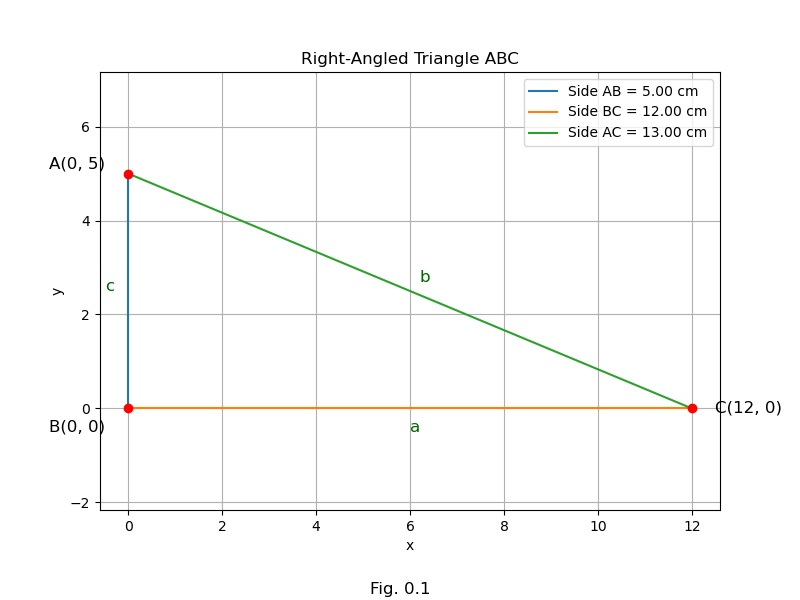
\includegraphics[width=\columnwidth, height=0.8\textheight, keepaspectratio]{figs/fig1.png}     
\end{frame}


\end{document}
